%!TEX root = ../dissertation.tex

\chapter{Background}
\label{chapter:background}
This chapter presents the background necessary to comprehend the developed work. The first section
presents the related work relevant regarding to solve the challenges of converging the Internet of
Things and the Utility Computing. The following sections presents a description of the concepts
that composes the basis of our work.

% Related Work
\section{Related Work}
\label{section:related_work}
Recently a lot of research and effort has been dedicated to solve these existing problems. In this
section we will present a summary of the most relevant work that relates to the Internet of Things and the utility computing:

% Service Delivery
\subsection{Service Delivery}
\label{sub:service_delivery}
As referred in Section~\ref{section:motivation}, current \gls{IoT} solutions are delivered in a physical
and isolated manner, which makes its service delivery model an inefficient and unscalable process.
In order to turn the service delivery of \gls{IoT} solutions more efficient and scalable, cloud service
delivery models are being developed based on the existing layers of the cloud architecture \cite{zhang2010cloud}:
\textit{a) \gls{IaaS}} refers to the provisioning of infrastructure resources on-demand - e.g. \glspl{VM},
storage and network. \textit{b) \gls{PaaS}} refers to providing platform layer resources such as operating
system support and software development frameworks. \textit{c) \gls{SaaS}} refers to providing on demand
application over the Internet.

% Soldatos
\subparagraph{Soldatos} et al. \cite{soldatos2012convergence} presented the idea of converging the IoT
and the utility computing in the cloud. The proposed architecture is the core concept of the OpenIoT
Project\footnote{http://openiot.eu}, and is based on CoAP \cite{shelby2014constrained} and linked data.
The cloud is used at infrastructure level, which allows to measure the utility of the services provided
by inter-connected objects.
% Distefano
\subparagraph{Distefano} et al. \cite{distefano2012enabling} proposed a conceptual architecture by
mapping various elements in both cloud and IoT to the three layers of cloud architecture (\gls{PaaS},
\gls{SaaS} and \gls{IaaS}). In this proposal IoT resources are provided voluntarily by their owners,
while management functions - such as node management and policy enforcement - are viewed as peer
functions of cloud infrastructure management. A \gls{PaaS} module is responsible to mashup IoT resources
and cloud infrastructure (\gls{IaaS}) for applications, which are delivered through \gls{SaaS}.
% CloudThings
\subparagraph{CloudThings} \cite{zhou2013cloudthings} is an architecture that uses a common
approach to integrate Internet of Things and Cloud Computing. The proposed architecture is an online
platform which accommodates \gls{IaaS}, \gls{PaaS}, \gls{SaaS} and allows system integrators and
solution providers to leverage the complete application infrastructure for developing, operating
and composing applications and services.
% IoT PaaS
\subparagraph{Li} et. al \cite{li2013efficient} proposed IoT PaaS, a cloud platform that supports
scalable IoT service delivery. Solution providers are able to deliver new solutions by leveraging
computing resources and platform services - domain mediation, application context management, etc.
- on the cloud. The proposed architecture aims to enable virtual vertical service delivery, for that
it has a multi-tenant nature which is designed to help at the isolation of the environments of
different solutions.\\

Although great progress was achieved regarding the improvement of service delivery for \gls{IoT}
solutions, most of the work still are in a conceptual stage. What is certain is that cloud service
delivery models will be the foundation for the service delivery models for \gls{IoT}.

% Data Storage Performance
\subsection{Data Storage Performace}
\label{sub:data_storage}
Since that data storage and retrieval in the cloud had specific requirements, cloud providers started
to implement their own solutions.

\subparagraph{Google Big Table, Facebook Cassandra and  Amazon Dynamo} \cite{chang2008bigtable} \cite{lakshman2010cassandra}
\cite{decandia2007dynamo} are key-value stores - \gls{NoSQL} databases - that has the ability to horizontally scale - i.e,
distribute both data and load of simple operations through many servers - but it has a weaker concurrency model
than the ACID transactions of most \glspl{RDBMS} systems \cite{cattell2011scalable}.

\subparagraph{\gls{PIQL}} \cite{armbrust2010piql} is a SQL-like API built to run on top of existing
performance predictable key-value stores, that provides many of the benefits of using a traditional
\gls{RDBMS}, such as the ability to express the queries in a declarative way, automatic data
parallelism, physical data independence and automatic index selection and maintenance, all while
maintaining the low latency guarantees on application performance that come from the underlying
key-value store.\\

Recently, some progress has been reached as regards scalable storage for \gls{RDBMS} systems. Although most
of the works still are in development, it is possible to highlight some solutions that are in a more
mature state.

\subparagraph{MySQL Cluster} \cite{ronstrom2004mysql} is an in-memory clustered distributed \gls{RDBMS}.
Compared with the MySQL implementation it works by replacing the InnoDB engine with the NDB - a proprietary
distributed layer from MySQL. MySQL Cluster is built on top of a shared-nothing architecture and includes
features such as failover, node recovery, synchronous data replication and no single point of failure.
MySQL Cluster seem to be the solution that scales to more nodes than other \gls{RDBMS} - 48 is the limit.
However, it was reported that after scaling up to a few dozen nodes it starts to running into
bottlenecks \cite{bunch2010evaluation}.

\subparagraph{VoltDB} \cite{stonebraker2013voltdb} is a \gls{RDBMS} designed for performance and scalability.
VoltDB assumes a multi-node cluster architecture where the tables are partitioned over multiple servers.
Tables can be replicated over servers - e.g. for fast access to data - shards are always replicated -
to recovery the data in case of a node crash - and database snapshots are supported. Currently some
features still are missing - online schema changes are limited and asynchronous \gls{WAN} replication and
recovery are not yet implemented - but in its current implementation VoltDB already presents some
features that improves the performance of SQL execution, as result the number of nodes that are needed
to support a given application load can be reduced in a significant way.

% Low-latency Interaction
\subsection{Low-latency Interaction}
\label{sub:low_latency_interaction}
Finding a general solution for the low-latency requirement of \gls{IoT} systems is not a easy task.
Since there are several application domains, it is natural that each application domain requires
that different values for network latency and data transmission latency are guaranteed.
% Talk about fog computing

 % Concepts
\section{Concepts}
\label{sec:Concepts}
This section presents the basics concepts that are relevant in the developed work. First, we start by
introducing the Fog Computing platform. Then, we present a description of the middleware platforms that
supports the \gls{RFID} technology. To end, we conclude with a brief description of the \glspl{LXC} technology
and the configuration management tools.

% Fog Computing
\subsection{Fog Computing}
\label{sub:fog_computing}
The Fog Computing \cite{bonomi2012fog} is a platform that aims to bring the cloud close to the ``Edge
of the Network''. By extending the cloud close to the ground, the Fog will be able to meet the requirements
of several applications that the traditional cloud is not able to accomplish. The most notable case
is the Internet of Things, that requires mobility support, geo-distribution in addition to location
awareness and low latency. The Fog achieves that by virtualizing the computing, storage and network
services between end devices and the traditional data centers in the cloud, that are not exclusively
located at the edge of the network.\\

% Fog Computing Infrastructure
\begin{figure}[ht!]
  \centering
  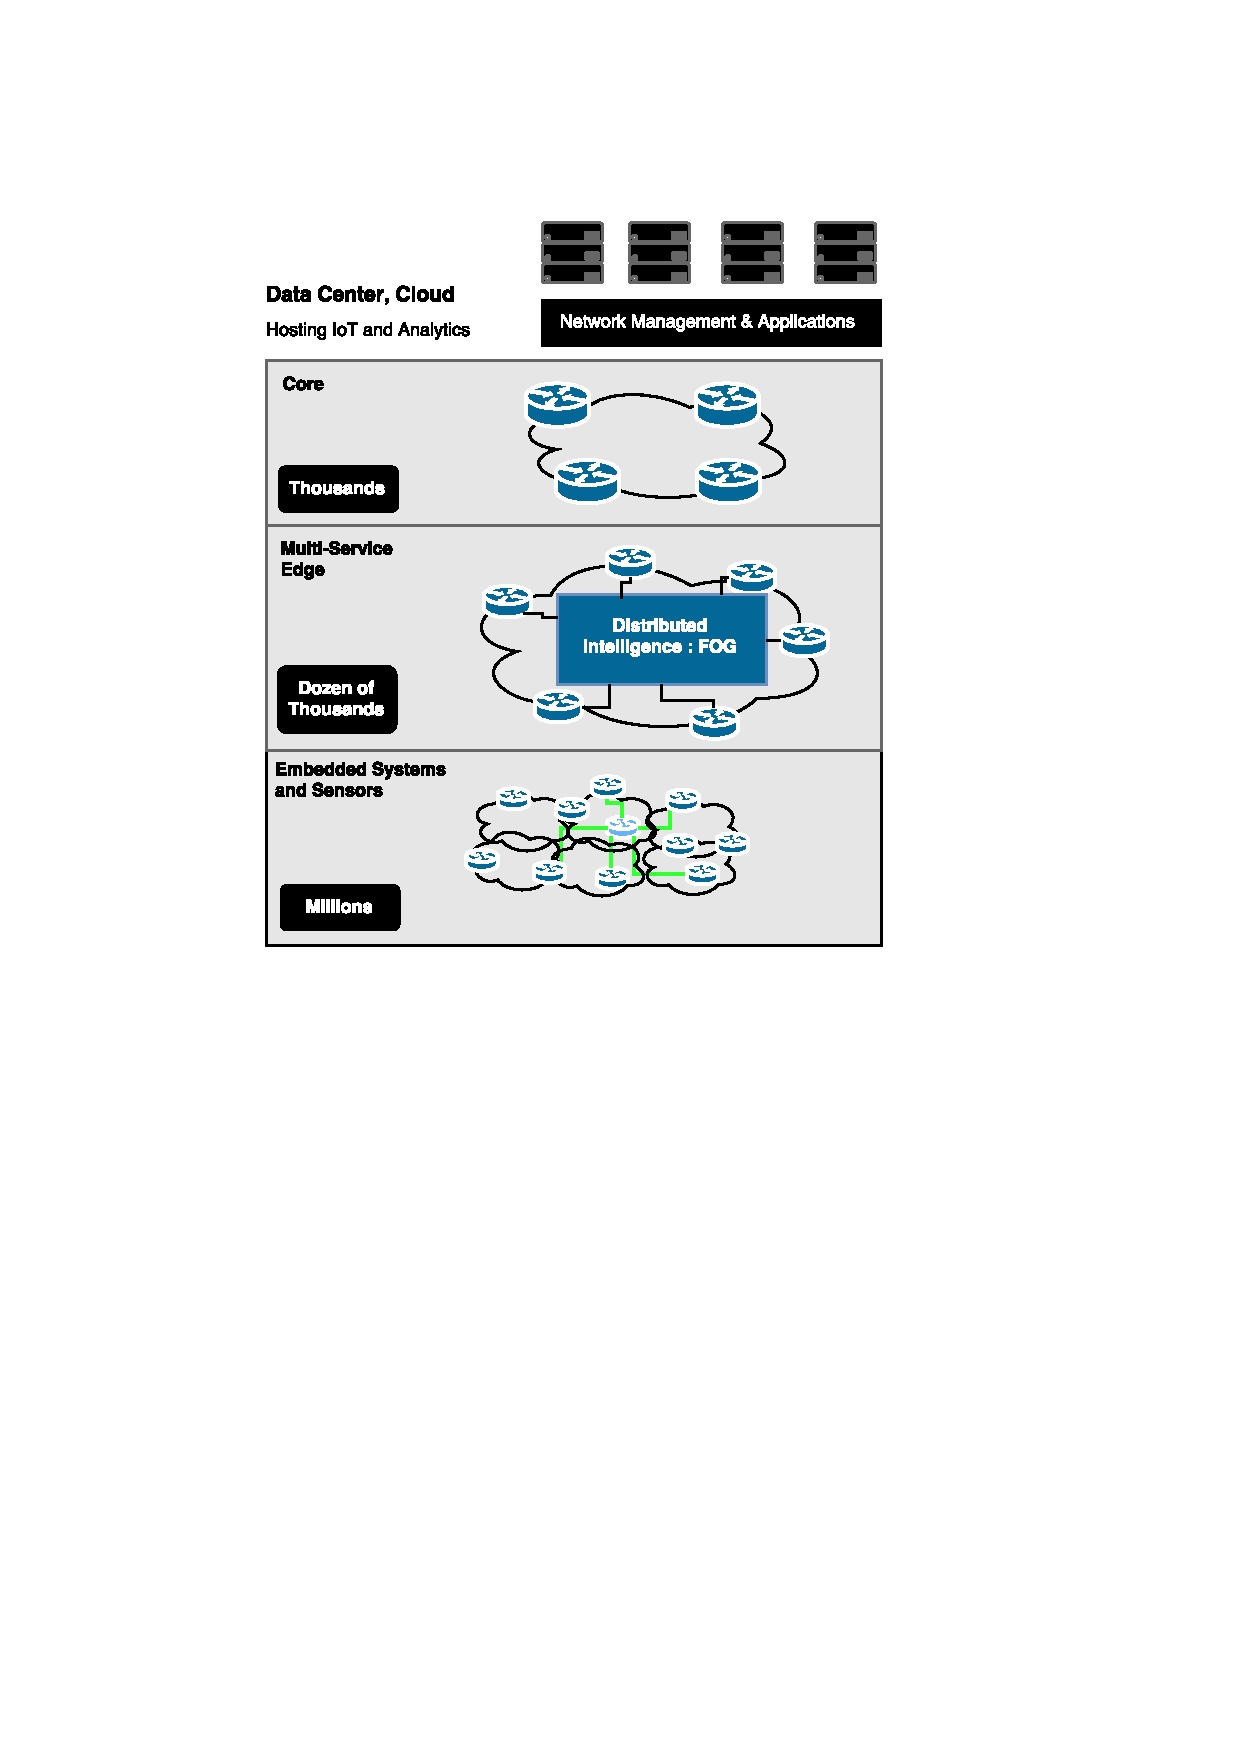
\includegraphics[width=.9\textwidth]{./images/fog_architecture}
  \caption{The Internet of Things and Fog Computing (Bonomi et. al (2012)).}
  \label{fig:fog_architecture}
\end{figure}

Figure~\ref{fig:fog_architecture} presents the architecture of the Fog Computing platform.
The distributed infrastructure of the Fog is composed of heterogeneous resources that must be managed
in a distributed way. The infrastructure comprising of several players, covering from data centers,
core of the network, edge of the network and end devices. The \textit{Embedded Systems and Sensors} is
the lowest layer of the Fog and it is responsible to perform \gls{M2M} interaction. It collects and
process the data from the sensors, issues controls to the actuators and also filters the data that
is locally consumed and send the rest to the higher layers. The \textit{Multi-Service Edge} and
\textit{Core} layers are responsible to perform visualization and reporting - e.g. \gls{H2M} interaction -
as well to deal with systems and processes (\gls{M2M}).\\

Since that interaction between the different layers can range from seconds - e.g. low-latency real-time
analytics - to days - transactional analytics - the Fog must support several types of storage, from
ephemeral storage at the lowest layers to semi-permanent at the highest layer. It is important to point
that the higher the tier, the geographical coverage is wider and the time scale is larger \cite{bonomi2014fog}.
The global coverage is given by the Cloud, which acts as a central repository for the persistent data
and that is used to perform business analytics.

\subsection{RFID Middleware}
\label{sub:rfid_middleware}
The \gls{RFID} middleware is the component of a \gls{RFID} system that sits between the low level
components - e.g. readers and tags - and the business client application - e.g. \gls{ERP} systems.
The next paragraphs describes the EPCglobal, a framework that provides standardized interfaces that
isolates hardware vendors from business applications, and Fosstrak, a open-source \gls{RFID}
middleware platform that implements the GS1 \gls{EPC} Network standards.

% GS1 EPC Network
\subparagraph{GS1 EPCglobal Architecture}
\label{subp:epc_network}
GS1\footnote{http://www.gs1.org} is an organization that is responsible for the development and maintenance of standards for
supply chain. One of the standards developed by GS1 is the \gls{EPC}, which is a unique serial identifier
for \gls{RFID} tags. GS1's subsidiary EPCglobal Inc.\footnote{http://www.gs1.org/epcglobal} created
the EPCglobal Architecture Framework, that currently is the standard for \gls{RFID} platforms.
Figure~\ref{fig:epc_architecture} presents the architecture of the EPCglobal framework.\\

% EPC Architecture
\begin{figure}[ht!]
  \centering
  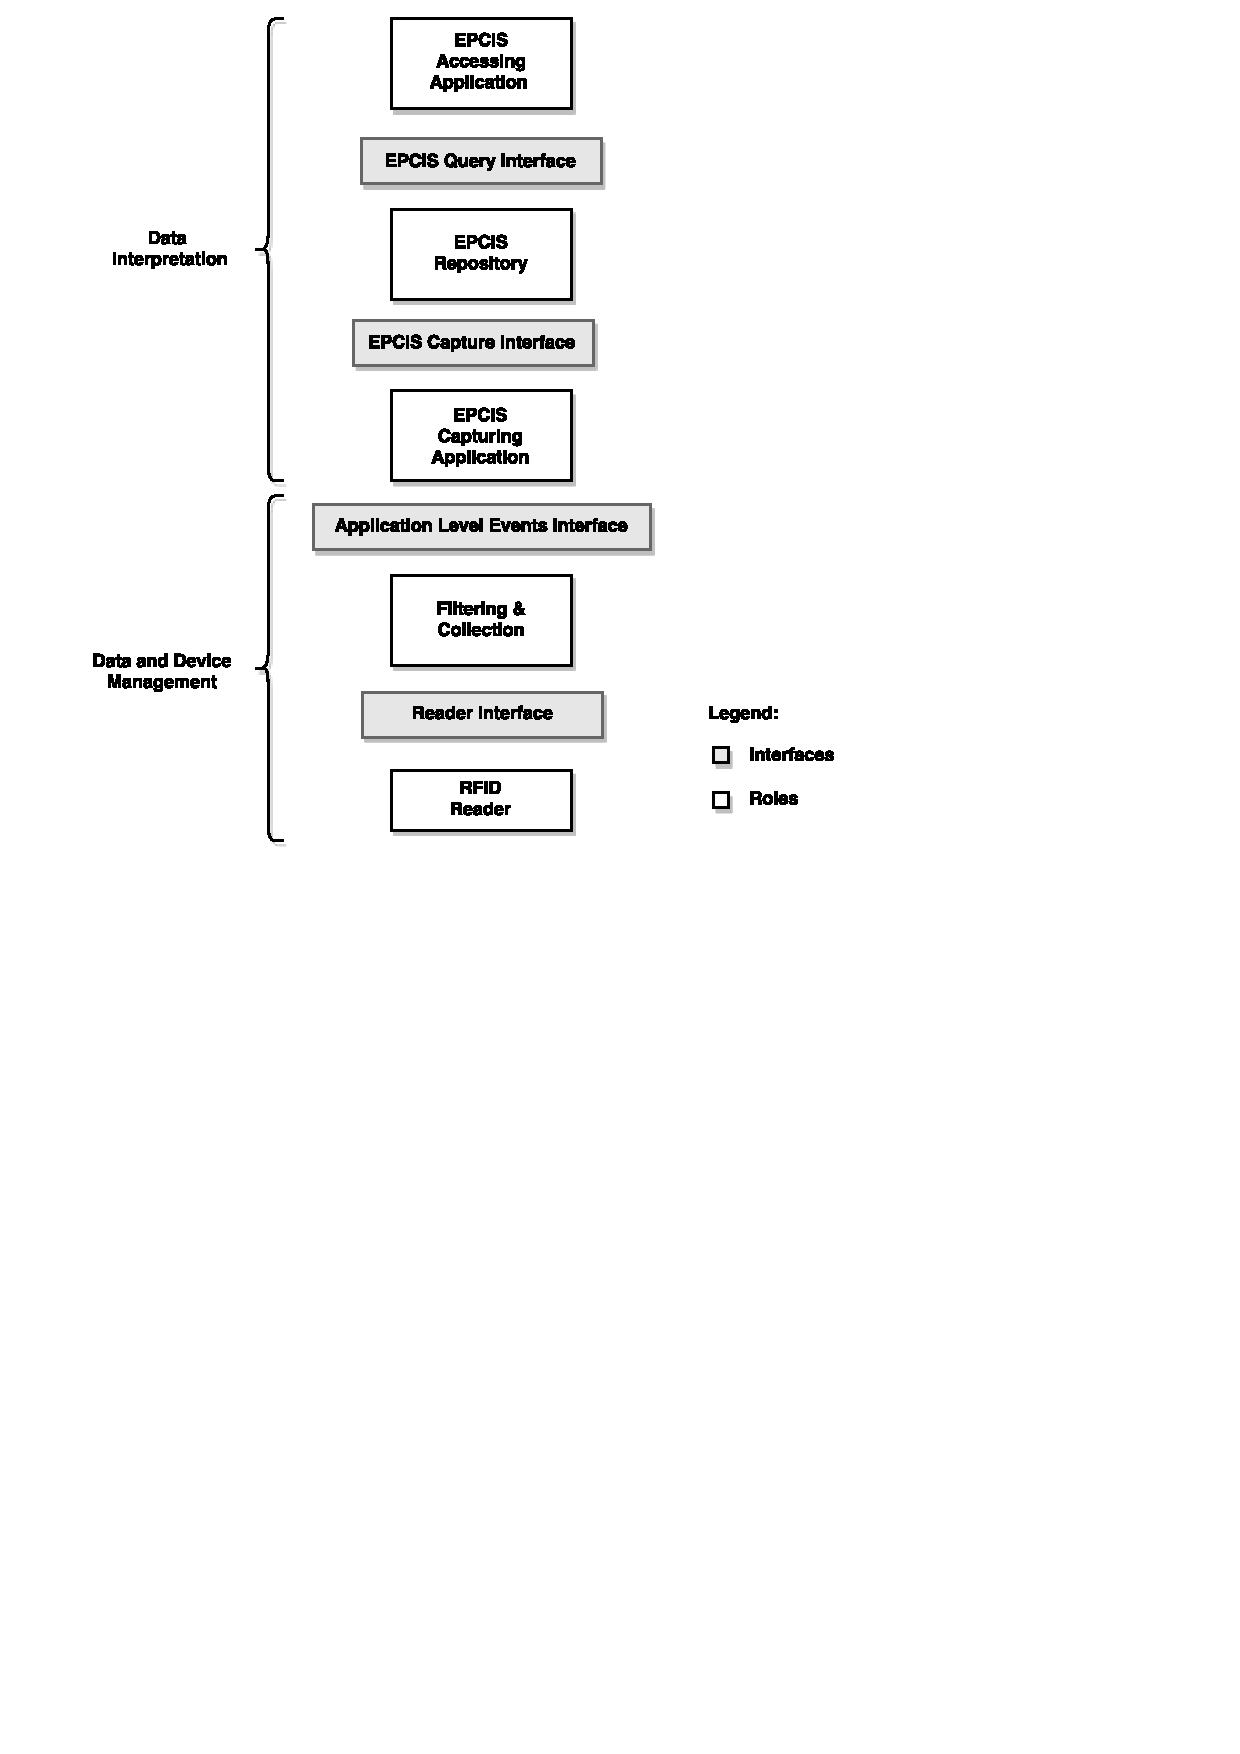
\includegraphics[width=.8\textwidth]{./images/EPCGlobal_architecture}
  \caption{GS1 EPCGlobal Architecture Framework.}
  \label{fig:epc_architecture}
\end{figure}

The framework\footnote{For more information about the EPCglobal Framework Architecture standard, the
full documentation is available at \href{http://www.gs1.org/gs1-architecture}{GS1 standards}} has a
set of standardized interfaces that enables the interchange of information between entities:

% EPC Architecture components
\begin{itemize}
  % Reader Interface
  \item Reader Interface provides the interfaces that must be implemented by the \gls{RFID} readers.
  The \gls{LLRP} standard provides interfaces that allows to control all the aspects of \gls{RFID}
  reader operation.
  % Filtering & Collection
  \item Filtering \& Collection is the module that coordinates the \gls{RFID} readers that are in the
  same physical space and also abstracts the readers from the upper layers. It allow to execute read
  and write operations on tags. Furthermore, it is responsible to filter, aggregate and grouping the
  raw tag data when requested.
  % Filtering & Collection Interface
  \item \gls{ALE} Interface defines the control and delivery of filtered and collected data from the
  Filtering \&  Collection to the \gls{EPCIS} Capturing Application. The \gls{ALE} are a selection of
  the events that are meaningful for the client applications.
  % EPCIS Capture Application
  \item EPCIS Capture Application supervises the operation of the lower EPC layers, and provides
  business context based on information involved in the execution of a particular step of a business
  process.
  % EPCIS Repository
  \item EPCIS Repository is the module where all the business events generated by EPCIS Capturing
  Applications are stored to be later be accessed by EPCIS Accessing Application. The EPCIS Query
  Interface defines how client applications can retrieve information from the repository.
\end{itemize}

% Fosstrak
\subsection{Fosstrak Platform}
\label{sub:fosstrak}
The Free and Open-Source for TRAcK and trace (Fosstrak), designed and implemented by Floerkemeier et
al. (2007), is an open source platform compliant with EPCglobal Network specifications, freely available
to any company and / or researcher that wants to use or develop on top of it. Figure 2.7 shows the architecture
with all the available modules. Comparing with EPCglobal architecture presented in Figure 2.6 the
Fosstrak platform covers all the “End User” components except the “Local ONS” module.

% Fosstrak Architecture
\begin{figure}[ht!]
  \centering
  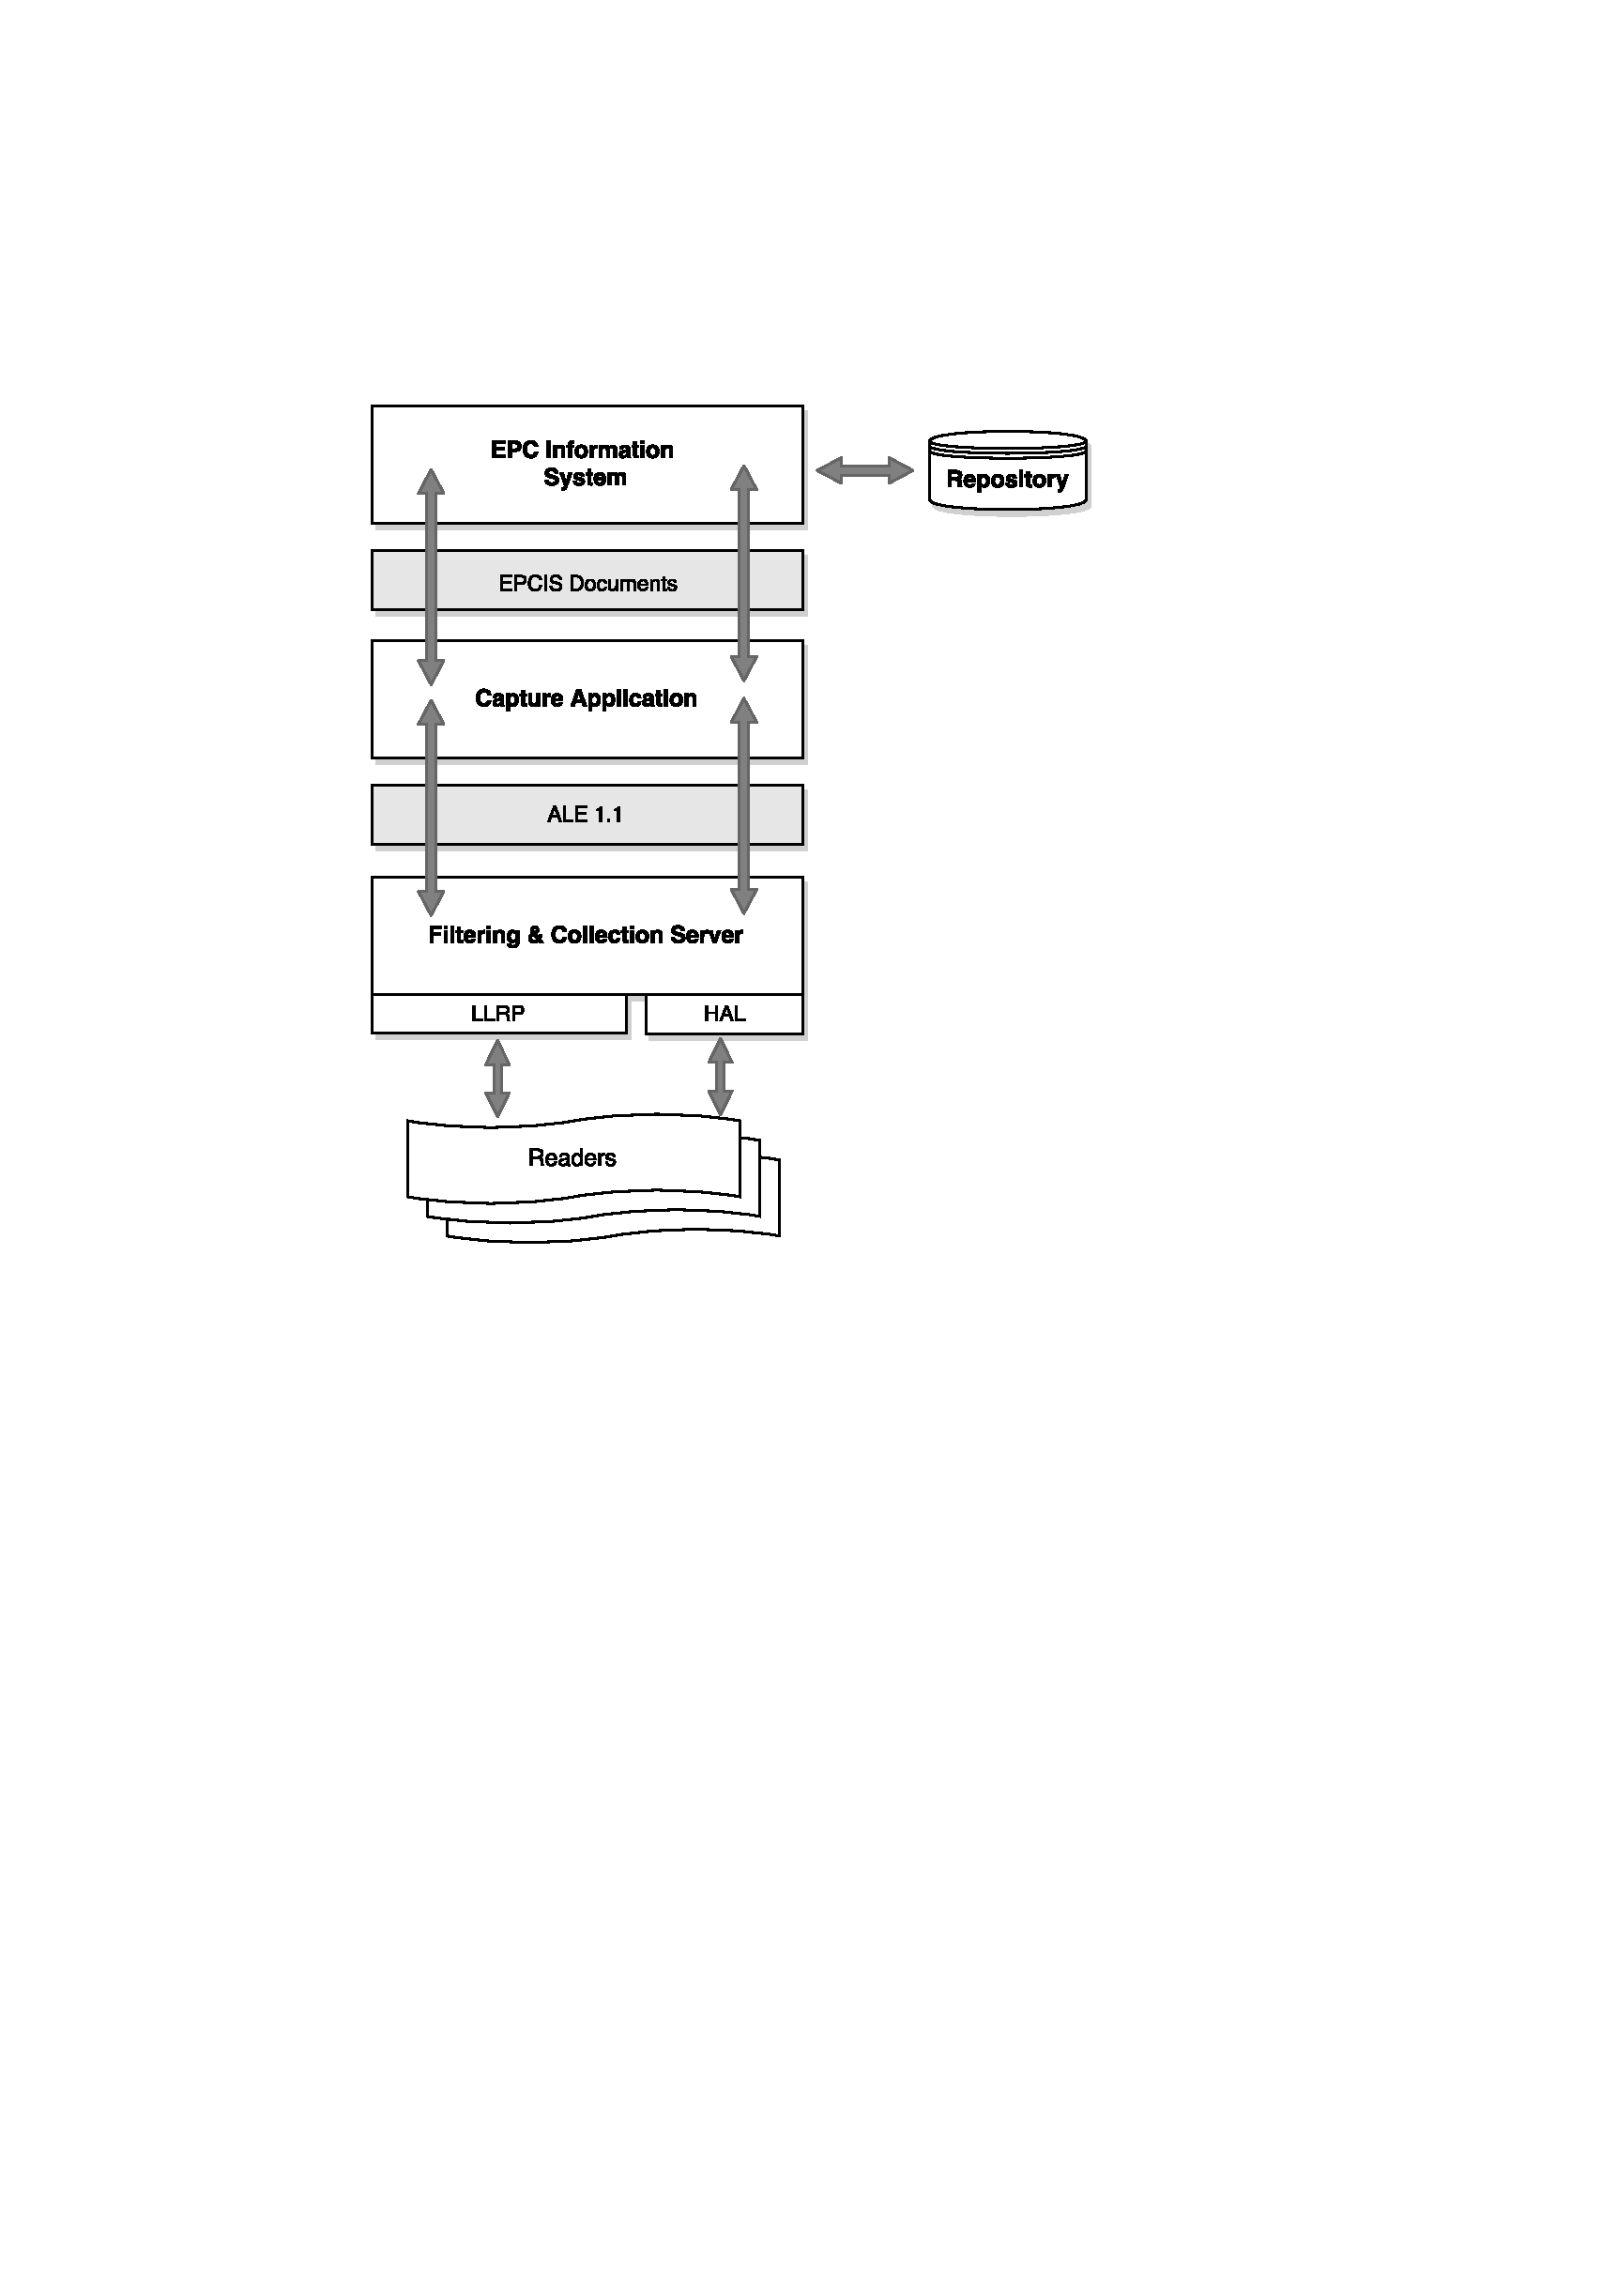
\includegraphics[width=.725\textwidth]{./images/fosstrak_architecture}
  \caption{Fosstrak architecture.}
  \label{fig:fosstrak_architecture}
\end{figure}

% FC Server
\subparagraph{Filtering \& Collection Server}
FCServer is the module responsible to abstract the readers from the rest of the Fosstrak’s architecture.
It has two types of connections, one named Hardware Abstraction Layer (HAL) where it is possible to
develop a custom connection to each reader. And the LLRP connection to enable all LLRP complaint
readers to be connected to the middleware just by configuration. Internally, these readers are
LogicalReader instances and configured through a LRSpec document as defined by EPCglobal (2009).
Fosstrak implements the mechanism specified in EPCglobal (2009) to reduce the number of false readings
called Event Cycle. This mechanism is implemented in the Data Cleaning module where it is possible to
programmatically change the data cleaning strategy. The output of the Data Cleaning module is an
ECReport document that is sent to the Capture Application.

% Capture Application
\subparagraph{Capture Application}
Before a business event is sent to the EPCIS Repository, the capture application
may request more information about the identified object to external services. For example, a
specific product is identified in the reader deployed in the warehouse’s entrance, the capture
application can now request information about this product from the ERP system to know if it is an
expected product from a supplier or a returned product from a costumer. Regarding its implementation,
the Capture Application is built on top of a Drools1 engine where rules can be specified in the form of:
“when” a tag is received from the warehouse entrance, “then” do “this”. Unfortunately, all rules must
be predefined and can not be changed during runtime if needed.

% EPCIS
\subparagraph{EPCIS}
This module is EPCglobal-certified meaning that all Fosstrak EPCIS modules and interfaces are
verified by the EPCglobal organization. Additionally, it implements a Query Callback Interface on which
those events matching a specific criteria are sent. Criterias are defined through subscriptions that
must be previously configured by an EPCIS Accessing Application. The EPCIS Repository stores the following
information for each business event: a) Read Point where the read was taken, for instance in the warehouse’s
dock door; b) Business Location where the tag was identified, for instance the warehouse as a whole or other
specific area; c) Disposition specifies the state of the tagged object, for example the tagged product is
in the packaging area; and d) Business Step is the business action associated with the event, normally it
is used a verb to represent the action being taken, for instance entering the packaging area.

% Configuration Management Tools
\subsection{Configuration Management Tools}
\label{sub:cm_tools}


% Containers
\subsection{Containers}
\label{sub:containers}
Docker is an open source project to pack, ship and run any application as a lightweight container.
Docker containers are hardware-agnostic and platform-agnostic, this means that these containers can
run anywhere, from a laptop to a cloud instance. Since Docker is based in Linux Containers (LXC),
the virtualization is performed at operating-system level, di↵erent of hypervisor-based solutions where
the virtualization is performed at hardware- level. While the e↵ect of both types of virtualization
are similar, the virtualization at the operating-system level provides significant benefits compared
to hypervisor-based solutions. Docker containers are small, they have low memory and CPU overhead,
they also are portable between di↵erent virtualization environments.\\

Another benefit that Docker platform provides is the Docker Registry service, a public repository
that stores Docker images used to create the containers. In our solution we built the Docker images
of the Fosstrak modules and published them in Docker registry to later be used to create our containers.
